\section{Erweiterung}
\rhead{Erweiterung}
\subsection{Filterung}


Unser Programm erlaubt es die vorher beschriebene Radonr"ucktransformation
durchzuf"uhren. Durch die vorgegebene Radontransformation kann man nun
mit einem beliebigen Bild (hier Orginalbild(a)) die Radontransformation
durchf"uhren und erh"alt dann das transformierte Bild, welches
als Ausgangsbild f"ur die R"ucktransformation verwendet wird (hier
Radontransformation(b)).

\begin{figure}[ht!]\centering
	\subfigure[Orginalbild]{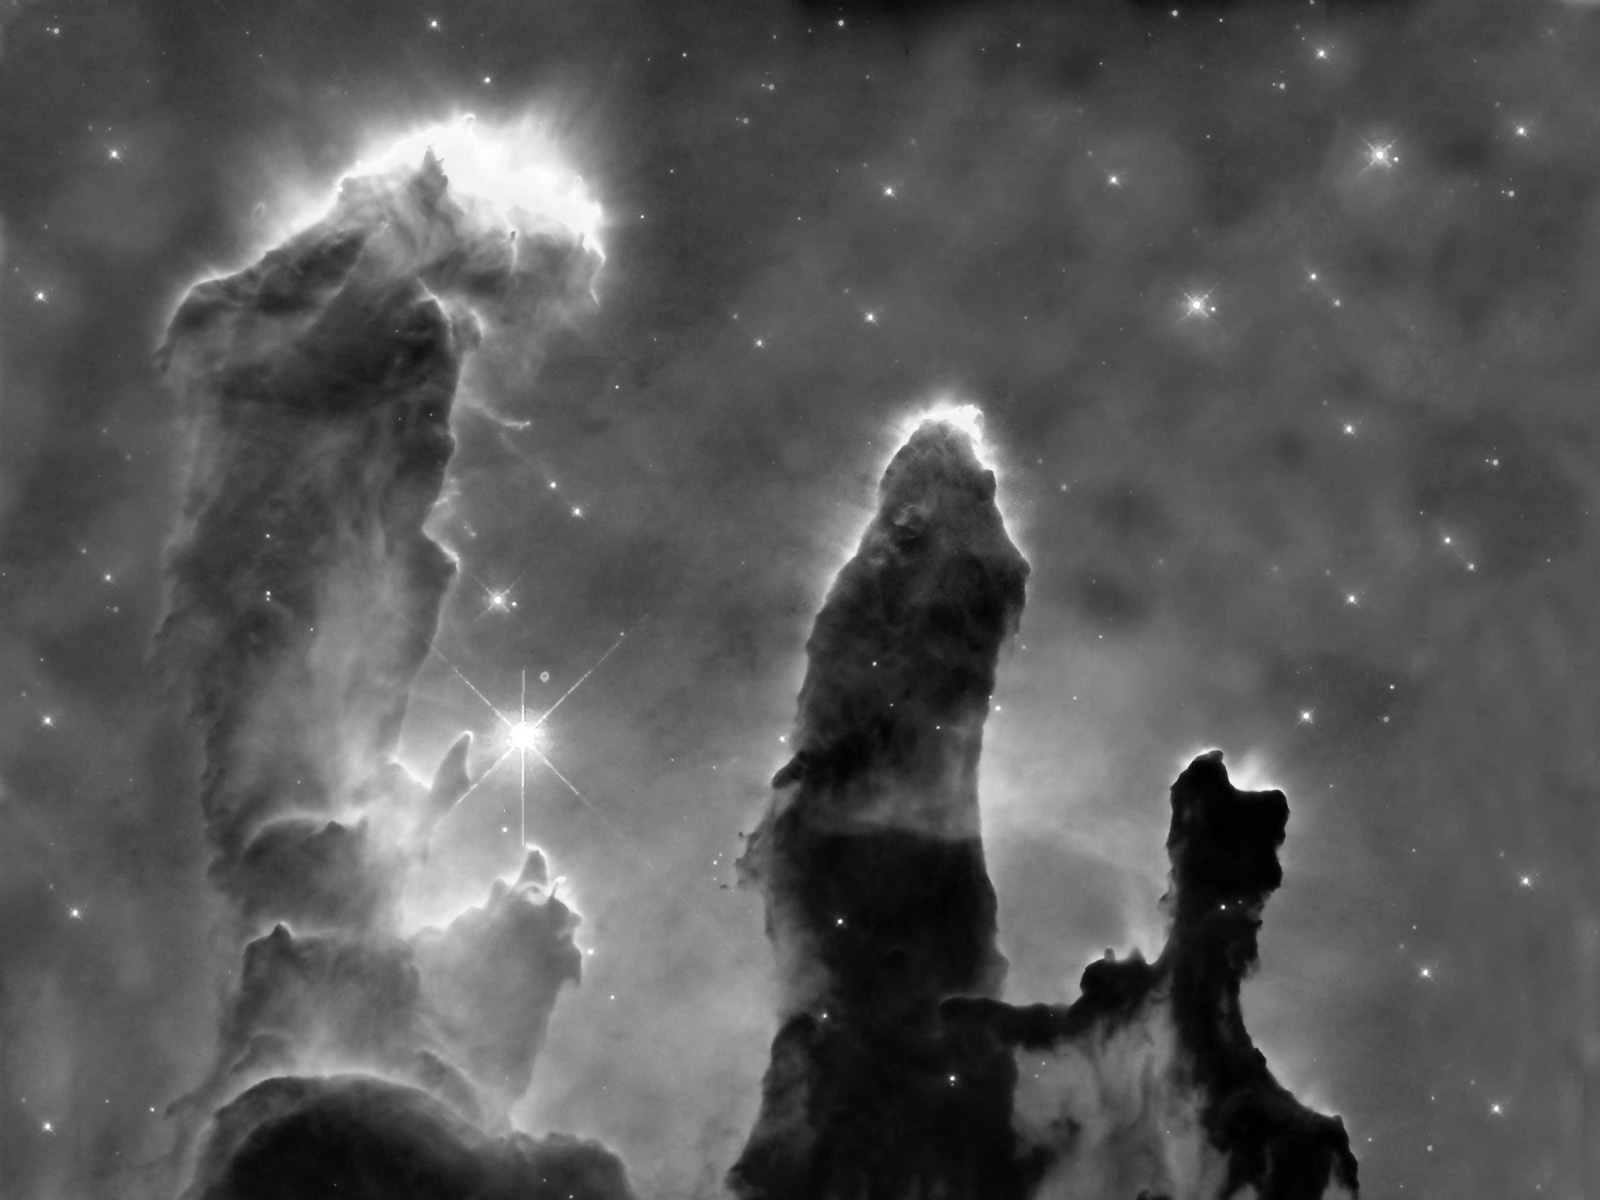
\includegraphics[width=0.4\textwidth]{radon/images/pocM.jpg}}
    \subfigure[Radontransformation]{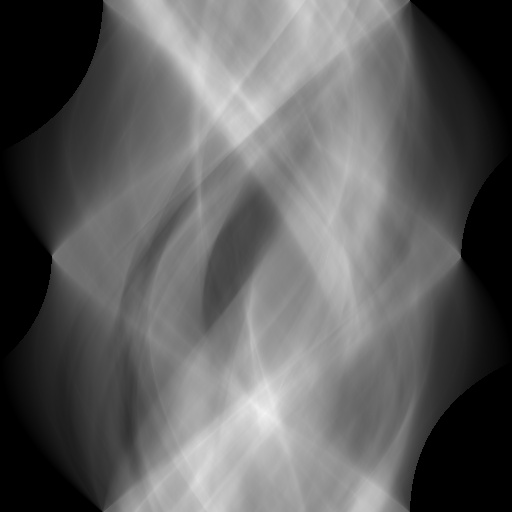
\includegraphics[width=0.3\textwidth]{radon/images/pocTF.jpg}}  
\end{figure}

Durch unsere R"ucktransformation k"onnen wir jetzt daraus wieder das
Orginalbild herstellen (hier R"uckprojektion(c). Das Orginalbild l"asst
\index{Ruckprojektion!R\"uckprojektion}
sich zwar deutlich erkennen, es hat aber viele helle Schatten, welche
durch Randeffekte der R"ucktransformation entstehen. Diese Stellen werden
Schatten genannt. Das Problem ist, dass sich die Cosinuskuven, welche
zu einem beliebigen Punkt im Bild geh"oren, sich mit Cosinuskurven von
anderen Punkten "uberschneiden, durch die Integration "uber die ganze
Kurve, werden dadurch viele Punkte zu Hell dargestellt.

Durch ein Fourierfilter k"onnen diese Schatten jedoch herausgefiltert
werden. Nach der Filterung des generierten Bildes erhalten wir daraus
das gefilterte Bild(d).

\begin{figure}[ht!]\centering
	\subfigure[R"uckprojektion]{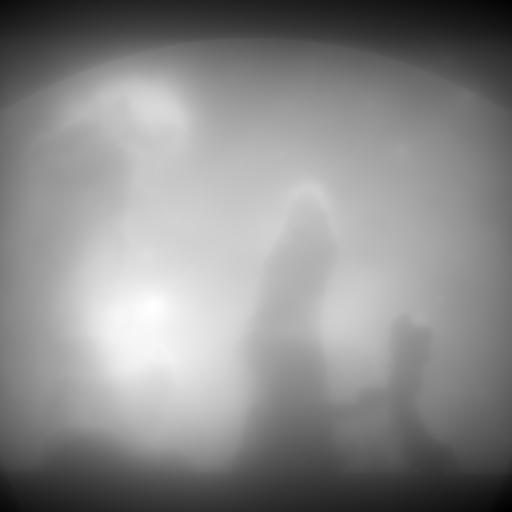
\includegraphics[width=0.3\textwidth]{radon/images/pocBTF.jpg}}
    \subfigure[Gefiltertes Bild]{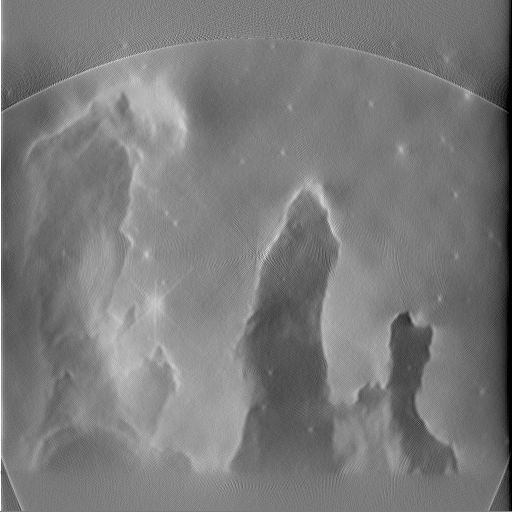
\includegraphics[width=0.3\textwidth]{radon/images/pocF.jpg}}
\end{figure}
\FloatBarrier

\subsection{Weitere Anwendungen der Radontransformation}

Durch die Radontransformation kann man auch Linien in einem Bild finden
und als Punkte darstellen. Unser Linie im Ausgangsbild(e) wird also als
Punkt in der Radontransformation(f) darestellt. Dies kann man jetzt
beispielsweise bei einem Barcodescanner verwenden oder auch in der
Bildverarbeitung, um Linien zu finden.

\begin{figure}[ht!]\centering
	\subfigure[Ausgangsbild]{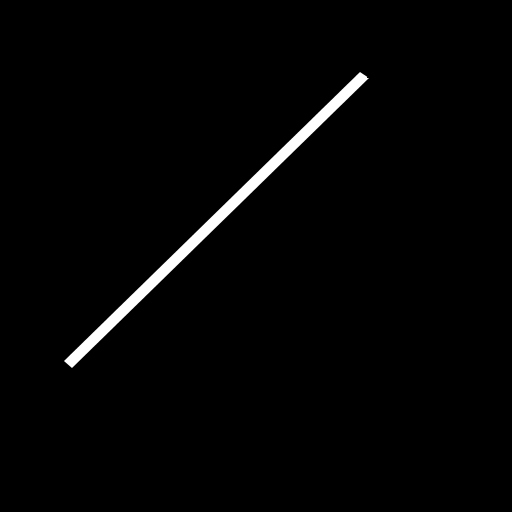
\includegraphics[width=0.4\textwidth]{radon/images/test2.jpg}}
    \subfigure[Radontransformation]{
\includegraphics[width=0.4\textwidth]{radon/images/test2TF.jpg}}
\end{figure}
\FloatBarrier
    
Durch die Transformation wird ein Barcode als eine Reihe von Punkten
auf einer horizontalen Geraden angeordnet. Die Durchmesser der Punkte
auf der in der Reihe verhalten sich zueinander wie die Breiten der
einzelnen Linien des Barcodes. Die Barcodescanner auf Smartphones
verwenden beispielsweise genau diese Beziehung.

Um die Visualisierung zu vereinfachen, haben wir das Bild des Barcodes(g)
\index{Barcode}
farblich invertiert, dies ist jedoch nicht unbedingt notwendig. in der
Radontransformation(h) kann man nun eine horizontale Reihe von hellen
Punkten erkennen, welche von rechts nach links gelesen dem Barcode(g)
entsprechen. Erh"oht man nun den Kontrast der der Radontransformation(h)
massiv so erh"alt man unser Kontrastbild(i) in welchem der Barcode in
form von Punkten wieder gut zu erkennen ist.

\begin{figure}[ht!]\centering
	\subfigure[Barcode]{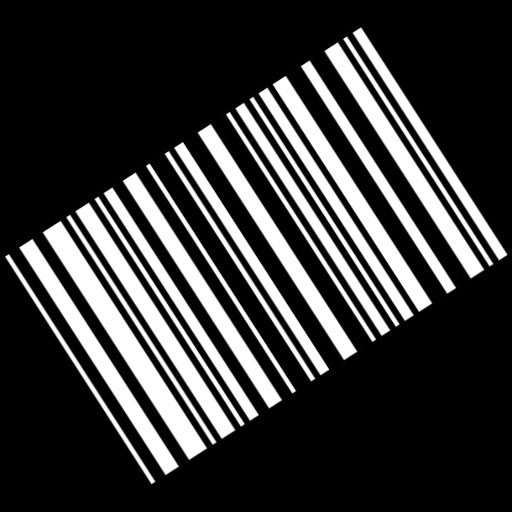
\includegraphics[width=0.3\textwidth]{radon/images/barcode3.jpg}}
    \subfigure[Radontransformation]{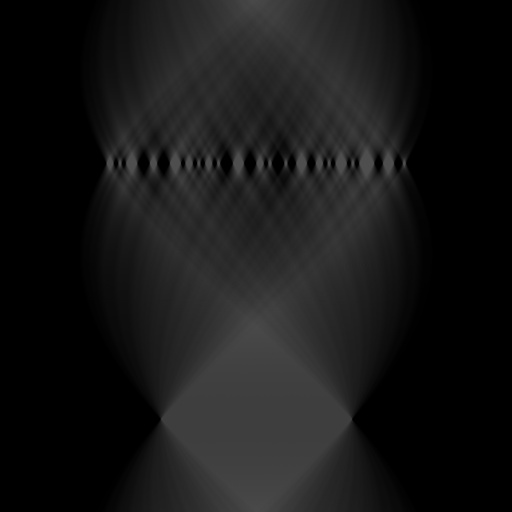
\includegraphics[width=0.3\textwidth]{radon/images/barcode3TF.jpg}}
    \subfigure[Kontrastbild]{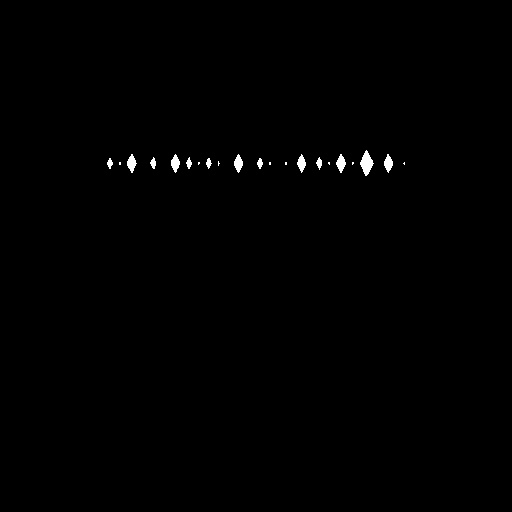
\includegraphics[width=0.3\textwidth]{radon/images/barcodeKONT.jpg}}
\end{figure}
\FloatBarrier
